\begin{figure}[H]
\centering
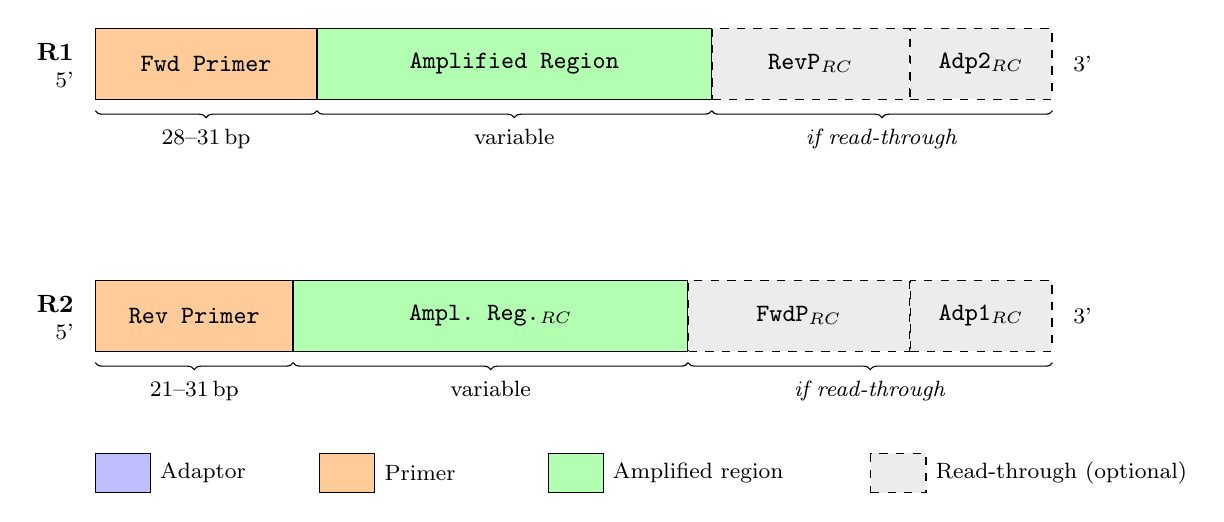
\begin{tikzpicture}[
    box/.style={draw, minimum height=0.9cm, text centered,
                font=\small\ttfamily, inner sep=3pt},
    adp/.style={box, fill=blue!25},
    prm/.style={box, fill=orange!40},
    amp/.style={box, fill=green!30},
    rth/.style={box, dashed, fill=gray!15},
    lbl/.style={font=\footnotesize},
]

% -------------------------------------------------------
% READ 1  (adapter is the priming site; read begins at forward primer)
% -------------------------------------------------------
\node[prm, minimum width=2.8cm, anchor=west] (r1fp) at (0, 0)     {Fwd Primer};
\node[amp, minimum width=5.0cm, anchor=west] (r1ar) at (r1fp.east){Amplified Region};
\node[rth, minimum width=2.5cm, anchor=west] (r1rp) at (r1ar.east){RevP$_{RC}$};
\node[rth, minimum width=1.8cm, anchor=west] (r1a2) at (r1rp.east){Adp2$_{RC}$};

% R1 label + direction
\node[anchor=east, font=\small\bfseries] at (-0.15, 0.15)  {R1};
\node[anchor=east, lbl]                  at (-0.15, -0.2)  {5'};
\node[anchor=west, lbl]                  at ([xshift=4pt]r1a2.east) {3'};

% Size annotations below R1
\draw[decorate, decoration={brace, mirror, raise=4pt}]
    (r1fp.south west) -- (r1fp.south east)
    node[midway, below=7pt, lbl] {28--31\,bp};
\draw[decorate, decoration={brace, mirror, raise=4pt}]
    (r1ar.south west) -- (r1ar.south east)
    node[midway, below=7pt, lbl] {variable};
\draw[decorate, decoration={brace, mirror, raise=4pt}]
    (r1rp.south west) -- (r1a2.south east)
    node[midway, below=7pt, lbl, text width=2.5cm, align=center]
        {\textit{if read-through}};

% -------------------------------------------------------
% READ 2  (adapter is the priming site; read begins at reverse primer)
% -------------------------------------------------------
\node[prm, minimum width=2.5cm, anchor=west] (r2rp) at (0, -3.2)    {Rev Primer};
\node[amp, minimum width=5.0cm, anchor=west] (r2ar) at (r2rp.east)  {Ampl.\ Reg.$_{RC}$};
\node[rth, minimum width=2.8cm, anchor=west] (r2fp) at (r2ar.east)  {FwdP$_{RC}$};
\node[rth, minimum width=1.8cm, anchor=west] (r2a1) at (r2fp.east)  {Adp1$_{RC}$};

% R2 label + direction
\node[anchor=east, font=\small\bfseries] at (-0.15, -3.05) {R2};
\node[anchor=east, lbl]                  at (-0.15, -3.4)  {5'};
\node[anchor=west, lbl]                  at ([xshift=4pt]r2a1.east) {3'};

% Size annotations below R2
\draw[decorate, decoration={brace, mirror, raise=4pt}]
    (r2rp.south west) -- (r2rp.south east)
    node[midway, below=7pt, lbl] {21--31\,bp};
\draw[decorate, decoration={brace, mirror, raise=4pt}]
    (r2ar.south west) -- (r2ar.south east)
    node[midway, below=7pt, lbl] {variable};
\draw[decorate, decoration={brace, mirror, raise=4pt}]
    (r2fp.south west) -- (r2a1.south east)
    node[midway, below=7pt, lbl, text width=2.5cm, align=center]
        {\textit{if read-through}};

% -------------------------------------------------------
% Legend
% -------------------------------------------------------
\begin{scope}[shift={(0, -5.2)}]
    \node[adp, minimum width=0.7cm, minimum height=0.5cm] (la) at (0.35, 0) {};
    \node[anchor=west, font=\footnotesize] at (0.7,  0) {Adaptor};

    \node[prm, minimum width=0.7cm, minimum height=0.5cm] (lp) at (3.2, 0) {};
    \node[anchor=west, font=\footnotesize] at (3.55, 0) {Primer};

    \node[amp, minimum width=0.7cm, minimum height=0.5cm] (lar) at (6.1, 0) {};
    \node[anchor=west, font=\footnotesize] at (6.45, 0) {Amplified region};

    \node[rth, minimum width=0.7cm, minimum height=0.5cm] (lrt) at (10.2, 0) {};
    \node[anchor=west, font=\footnotesize] at (10.55, 0) {Read-through (optional)};
\end{scope}

\end{tikzpicture}
\caption{Expected structure of paired-end reads from MiSeq amplicon
sequencing~\cite{illumina_miseq, goodwin2016}.
The sequencing primer binds\footnote{\textit{Annealing}: a short single-stranded
DNA oligonucleotide (the primer) binds to a complementary sequence on the template
strand via hydrogen bonds, positioning the polymerase to start copying from that
exact location.} within the adapter (Adp1 for R1, Adp2 for R2),
so the adapter itself is \emph{not} part of the sequenced read; sequencing begins
at the forward (R1) or reverse (R2) primer.
Solid borders: segments always present.
Dashed borders: segments that appear only when the read is long enough to
sequence through the full insert (read-through).
$_{RC}$: reverse complement.}
\label{fig:read-structure}
\end{figure}
